\documentclass[review]{elsarticle}
\graphicspath{ {./figures/} }
\usepackage{hyperref}
\usepackage{float}
\usepackage{verbatim} %comments
\usepackage{multirow}
\usepackage{apalike}
\usepackage{biblatex}
\usepackage{amsmath}
\addbibresource{ref.bib}
\restylefloat{figure}
\restylefloat{table}
\usepackage[ruled,vlined]{algorithm2e}
\renewcommand{\baselinestretch}{1.05}


% \journal{Expert Systems with Applications}
\makeatletter
\def\ps@pprintTitle{%
 \let\@oddhead\@empty
 \let\@evenhead\@empty
 \def\@oddfoot{}%
 \let\@evenfoot\@oddfoot}
\makeatother
% For ESWA journal you need to use APA style/

\begin{document}
\begin{frontmatter}
\title{\textbf{Survey of popular Link Prediction algorithms and heuristics}}
\author{Abhinav Kumar-180050003, Nimay Gupta-180050068, \\ Niraj Mahajan-180050069}

\begin{abstract}
Link Prediction is a key problem for network structured data. It has wide practical applications in social networks, citation networks, and so on. Given a snapshot of a social network, can we infer which new interactions can be added based on the structure of the graph? This question is answered by Link prediction. In this survey, we compare the performance of various heuristics based methods and some popular supervised algorithms in link prediction.
\end{abstract}
\end{frontmatter}


\section{Introduction}
\noindent Due to the increasing surge in the research on complex graphical models, a considerable attention is devoted to Social Networks and their properties. A social network is a graph where the nodes represent entities or people, and the edges represent a link or connection between them. An example of a social network is citation graphs, where scientists working under the same discipline are the nodes, while the edges represent a collaboration. \\
Link Prediction is defined as: \textit{Given a snapshot of a social network at time t, we seek to accurately predict the edges that will be added to the network during the interval from time t to a given future time t'} \cite{liben_nowell_paper}. In other words, we need to use the intrinsic features of a social network to define a measure of proximity or similarity between any two nodes, and thus predict the probability of a link between the two.
\section{Heuristic-based Methods}
\noindent There exist several heuristic-based approaches to compute the similarity in the Link-Prediction problem. These heuristics are very simple, easy to implement and perform surprisingly well. Although these heuristics are not rigorously proven, work has been done on theoritically justifying the performance of these algorithms \cite{theoretical_justification_heuristics} \\There exist many heuristic-based algorothms like Adamic-Adar, Katz Measure, Preferential Attachment, Common Neighbor, Resource Allocation, Jaccard's coefficient. In this section, we will analyse the performance of these heuristic based methods on several sample graphs.
\subsection{Common Neighbors}
\noindent This is one of the most straightforward heuristic that is employed in link prediction. The score for an edge between two nodes u,v is given by simply the number of common neighboring nodes they share \cite{common_neighbors}, that is,
\[score(u,v) = |\Gamma(u) \cap \Gamma(v)|\]
\subsection{Preferential Attachment}
\noindent Preferential Attachment has received considerable attention as a model of the growth of networks\cite{PA_1,PA2}. The idea behind this heuristic is that the probability of a node being involved in a new edge is proportional to the degree of that node. We define $\Gamma(x)$ as the set of all neighbors of node x. Hence the score for a link between two nodes u,v is given by 
\[score(u,v) = |\Gamma(u)|.|\Gamma(v)|\]
\subsection{Adamic Adar}
\noindent Common Neighbors can sometimes fail in the case of nodes with high degrees. For example in a Facebook social network, a lot of unrelated people follow celebrities. Adamic and Adar \cite{adamic_adar_paper} proposed a measure similar to the common neighbors, which takes care of such a case. Instead of simply computing the number of common neighbors, we compute a weighted sum, weighing rarer features more heavily. In our case, the rarity of a feature is proportional to the degree of the node.
\[score(u,v) = \sum_{w \in \Gamma(u) \cap \Gamma(v)} \frac{1}{log(|\Gamma(w)|)}\]
\subsection{Jaccard Coefficient}
\noindent Jaccard coefficient \cite{Jaccard} measures the probability that both x and y have a common neighbor, for a for all the neighbors that either x or y has. It is popularly known as the Intersection over Union index.
\[score(u,v) = \frac{|\Gamma(u) \cap \Gamma(v)|}{|\Gamma(u) \cup \Gamma(v)|}\]
\subsection{Katz Measure}
\noindent Katz \cite{katz_paper} defines a measure that directly sums over the collection of paths between two nodes, exponentially damped by path length.\\
For nodes u,v, define $\mathbf{paths^{\langle l \rangle}_{u,v}}$ as the set of all l-length paths between nodes u,v.
\[score(u,v) = \sum_{l = 1}^{\inf} \beta^l.|\mathbf{paths^{\langle l \rangle}_{u,v}}|\]
where $\beta > 0$ is a dampening parameter. Using the adjacency matrix A, we can get the Katz matrix by solving the infinite geometric progression, as $\mathbf{K} = (\mathbf{I} - \beta \mathbf{A})^{-1} - \mathbf{I}$.
\section{Node2vec}
\subsection{Random walk}
\noindent In node2vec \cite{node2vec_paper}, given a source node u, we simulate a random walk of fixed length l. Let $c_{i}$  denote the ith node in the walk, starting with $c_{0} = u$. Nodes $c_{i}$ are generated by the following distribution:
\[
    P(c_{i}=x | c_{i-1} = v) = \left.
\begin{cases}
\frac{\pi_{vx}}{Z},& \text{if} (v,x) \in E\\
0,              & \text{otherwise}
\end{cases}
\right\}
\]
where $\pi_{vx}$ is the unnormalized transition probability between nodes v and x
\subsection{Search bias $\alpha$}
\noindent The simplest way to bias our random walks would be to sample the next node based on the static edge weights $w_{vx}$ i.e., $\pi_{vx} = w_{vx}$ . (In case of unweighted graphs $w_{vx}$ = 1.) However, this does not account for the graph structure and also does not guide our search procedure to explore different types og neighbourhoods. 
We define a 2nd order random walk with two parameters \textit{p} and \textit{q} which guide the walk. Conider a random walk that just traversed (t,v) and resides at node v. The walk now needs to decide the next node so it evaluates the transition probabilities $\pi_{vx}$ on edges (v,x) leading from v. We set the unnormalized transition probability to $\pi_{vx} = \alpha(t,x) \cdot w_{vx}$ where
\[
    \alpha(t,x) = \left\{\begin{array}{lr}
        \frac{1}{p}, & \text{if} d_{tx} = 0\\
        1, & \text{if } d_{tx} = 1\\
        \frac{1}{q}, & \text{if } d_{tx} = 2
        \end{array}\right\}
\]
and $d_{tx}$ denotes the shortest path distance between nodes t and x. Intuitively, p and q controls how fast the walk explores and leaves the neighbourhood of starting node v.
\subsection{The node2vec algorithm}
% \includegraphics[width=1.44\textwidth]{Ne2vec.png}
% \vspace{-1.4in}
\begin{figure}[h]
    \centering
    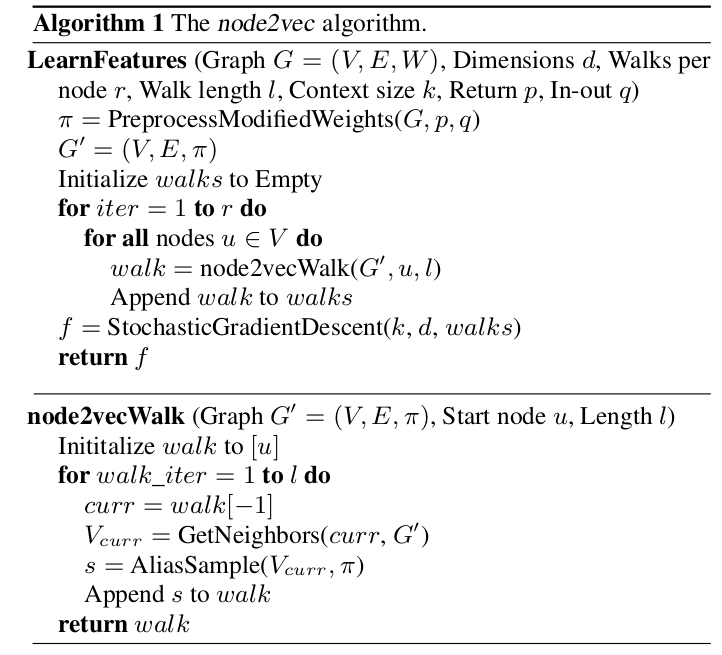
\includegraphics[width=1.\textwidth]{Node2vec.png}
    	\caption{Pseudocode for the Node2vec Embedding Generation Algorithm}
	    \label{fig:graphsage_pseudo}
\end{figure}
\noindent The pseudocode for node2vec, is given in Figure 1. In any
random walk, there is an implicit bias due to the choice of the start
node u. Since we learn representations for all nodes, we offset this
bias by simulating r random walks of fixed length l starting from
every node. At every step of the walk, sampling is done based on
the transition probabilities $\pi_{vx}$ . The transition probabilities $\pi_{vx}$ for the 2nd order Markov chain can be precomputed and hence, sampling of nodes while simulating the random walk can be done efficiently in O(1) time using alias sampling. The three phases of node2vec, i.e., preprocessing to compute transition probabilities, random walk simulations and optimization using SGD, are executed sequentially.
\subsection{Link prediction}
\noindent For the task of link prediction, we use the embeddings generated by node2vec algorithm to get the edge feature as $g(u,v) = f(u) o f(v)$ where the possible choices for binary operator $o$ are average, element-wise product, weighted-L1, weighted L2. Then we can use some fully connected neural network for predicting the edge score. Another possible way of edge prediction could be to use the cosine similarity between the embeddings of node u and node v as the edge score
% \newpage
\section{GraphSage}
\noindent The idea behind GraphSage\cite{graphsage_paper} embedding generation is to aggregate feature information from node's local neighbourhood(e.g. degrees, other node attributes) like message passing.
\subsection{Embedding Generation algorithm}
In this section, we describe the forward pass of the algorithm to generate the embeddings assuming some fixed weights for the learnable parameters. In particular, we use Mean aggregator which does not have learnable parameters and weight matrices $W_{k} \forall k \in \{1,..K\}$, which are used to propagate information between different layers of the model.
% \includegraphics[width=12cm, height=6cm]{figures/GSage.png}
\vspace{-1.4in}
\begin{figure}[h]
    \centering
    % \renewcommand{\thefigure}{1}
    % \begin{minipage}[c][1\width]{\textwidth}
    % 	\hspace*{-1.0in}
    	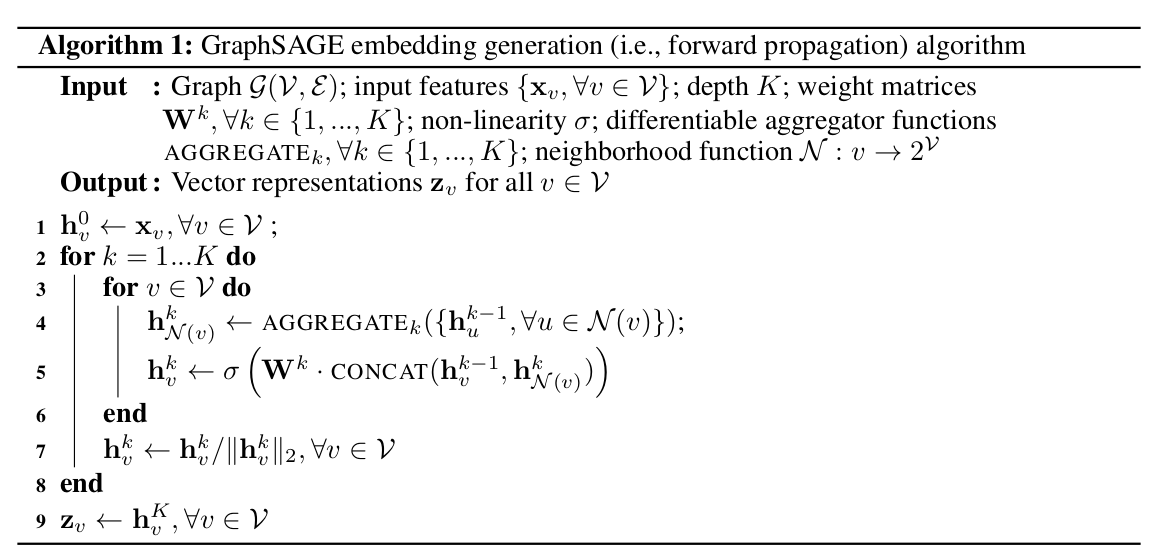
\includegraphics[width=1.\textwidth]{Gsage.png}
    % 	\null\vspace*{-98pt}
    	\caption{Pseudocode for the GraphSage Embedding Generation Algorithm}
	    \label{fig:graphsage_pseudo}
    % \end{minipage}
\end{figure}
Algorithm[1] describes the embedding generation process in the case where the entire graph, G = (V,E) and the features of all nodes $\mathbf{x}_{v} \forall v \in V$, are provided as input. Kth iteration in the outer loop describes the embedding generation for kth layer. $\mathbf{h}_{N(v)}^{k}$ denotes the aggregated representation of the neighbourhood of node $\mathbf{v}$. In our case, this aggregator function is Mean based i.e. the output of line4 above is the mean of node vectors of neighbours of $\mathbf{v}$. In next step, to generate the embedding for node v, aggregated representation is concatenated with features of layer k-1 and then a fully connected layer with nonlinear activation function $\sigma$ is applied on top of that.

\textbf{Neighbourhood definition.} In the code, we uniformly sample a fixed number of neighbours for each node rather than using all the neighbours to save on time complexity which otherwise would have been O(\|V\|).
\subsection{Learning the parameters}
\noindent For learning meaningful embedding for each node, we first train the network on cora dataset for node prediction task and then after learning the embedding, we train another network on top of that for link prediction. For node classification task, loss function is the regular cross entropy loss for classification.
\begin{equation}
    J_{G}(\mathbf{z}_{u}) = -y_{u}log(\sigma (\mathbf{z}_{u})) - (1-y_{u})log(1-\sigma (\mathbf{z}_{u})) 
\end{equation}
\subsection{Aggregator}
\noindent Since a node's neighbour have no natural ordering, the aggregator function must operate over a set of vectors. We describe here the mean and pooling aggregator.\\
\textbf{Mean Aggregator.} Our first candidate aggregator function is the mean aggregator, where we simply take the elementwise mean of the vectors in the set $\{\mathbf{h}_{u}^{k-1}, \forall u \in N(v)\}$. The mean aggregator is nearly equivalent of convolution in image domain.

\noindent \textbf{Pooling Aggregator.} This aggregator is both symmetric and trainable. In this \textit{pooling} apporach, each neighbour's vector is independently fed through a fully-connected neural network, following this transformation, an element-wise max-pooling operation is applied to aggregate information from the neighbour set:
\begin{equation}
    AGGREGATE_{k}^{pool} = max(\{\sigma (\mathbf{W}_{pool}\mathbf{h}_{u_{i}}^{k}+\mathbf{b}), \forall u_{i} \in N(v)\})
\end{equation}
where $max$ is the elementwise max operator and $\sigma$ is a non-linear activation function. In principle, before max-pooling, the function applied could be arbitrarily complex but here we focus on single layer neural network
\section{Evaluation}
\begin{table}[H]
\hspace*{-1.2in}
    \centering
    \begin{tabular}{ |p{1.5cm}|p{1.6cm}|p{1.5cm}|p{1.5cm}|p{1.7cm}|p{1.5cm}|p{1.5cm}|p{1.5cm}|p{1.5cm}|p{1.7cm}|  }
 \hline
 \multirow{2}{0.1cm}{Dataset} & \multirow{2}{3cm}{Evaluation \\ Method} & \multicolumn{7}{c|}{Algorithm} \\
 \cline{3-9}
  &   & Adamic \newline Adar & Common \newline Neighbor & Preferential \newline Attachment & Katz \newline Measure & Logistic\newline Regression & node2vec & GraphSage \\
 \hline
  \multirow{2}{*}{Facebook} & MAP & \textbf{0.726}   & 0.719   &  0.112  &  0.698  & 0.694 & 0.663 & ------------ \\
 \cline{2-9}
 & MRR & \textbf{0.875}   & 0.872   &  0.242  & 0.860   & 0.849 & 0.813 & ------------ \\
 \hline
 \multirow{2}{*}{Celegans} & MAP & 0.453   & \textbf{0.525}   &  0.304  &  0.446  & 0.453 & 0.400 & ------------ \\
 \cline{2-9}
 & MRR & 0.584   & \textbf{0.653}   &  0.443  & 0.583   & 0.587 & 0.530 & ------------ \\
 \hline
 \multirow{2}{*}{arXiv mini} & MAP & 0.814   & \textbf{0.831}   &  0.077  &  0.759  & 0.212 & 0.741 & ------------ \\
 \cline{2-9}
 & MRR & 0.922   & \textbf{0.936}   &  0.173  & 0.886   & 0.319 & 0.863 & ------------ \\
 \hline
 \multirow{2}{*}{cora} & MAP & 0.637   & \textbf{0.684}   &  0.169  &  0.500  & 0.466 & 0.405 & 0.01 \\
 \cline{2-9}
 & MRR & 0.664   & \textbf{0.713}   &  0.187  & 0.549   & 0.522 & 0.447 & 0.02 \\
 \hline
\end{tabular}
    \caption{Performance of various link predictors on several datasets. Bold entries represent the best performance.}
    \label{tab:results}
\end{table}
\paragraph{\textbf{Datasets}} In our analysis we have used four datasets to compare various LP algorithms - Facebook \cite{facebook_paper}, Celegans \cite{celegans_paper}, arXiv \cite{arxiv_paper}, cora \cite{cora_paper}. The facebook graph is social network, while arXiv and cora are citation graphs. C-elegans is a graph of neurons and synapses in C. elegans, a type of worm. we have used a reduced form of the arXiv graph (3000 nodes out of 10000).
\paragraph{\textbf{Performance of Heuristics}} We observe that Common Neighbors gives us the best results for cora, arXiv and celegans graph, while adamic adar gives the best results for the facebook graph. This is because adamic adar weights the score according to the degree of the common neighbor. Hence this shield our score from being influenced by celebrity nodes. Such nodes can be frequently occurring in the facebook graph, but will be less frequent in citation graphs as researchers have an additional hierarchies of fields, and subfields when they collaborate with others. Also, celebrity nodes in case of synapses (celegans) are also rare, since they occur at major synaptic junctions. Hence, common neighbors outperform adamic adar. \\
Preferential Attachment performs poorly as it is based on linking highly (socially) active nodes. This is a bad measure since it is improbable that an edge can be established between any two random nodes, just because they are socially active. For example it is absurd to say that two researchers, one in Computer Vision and one in Earth Science, will collaborate on a project.  \\
\paragraph{\textbf{Performance of node2vec and GraphSage}}
We observe that node2vec gives sub optimal results as compared to the heuristic based approaches, while GraphSage gives really bad results. Note that GraphSage requires intrinsic features as well and hence it is run only on the Cora dataset. Another observation to be noted is that the embeddings obtained using GraphSage give an 86.20\% accuracy for node classification. This proves that the embeddings are sensible and contain valuable information regarding the nodes. But since the graph is extremely sparse (~0.04 test fraction) the embeddings contain only the nodes' intrinsic information, and fail to extract the neighborhood information, or the edge-similarity information. This makes it difficult to train a logistic regression on the embeddings obtained from such sparse graphs. 
\section{Conclusion}
\noindent The heuristic based methods like common neighbors, adamic adar and katz measure are simple but extremely powerful, since they gave a performance which was at par, if not better, than the supervised methods. \\
GraphSage does not seem to work well on extremely sparse graphs as it is not able to extract neighborhood information in such cases and has to rely on the intrinsic features of nodes. \\

\newpage
\printbibliography
\end{document}